\documentclass[conference]{IEEEtran}
\IEEEoverridecommandlockouts

\usepackage{amsmath,amssymb}
\usepackage{siunitx}
\usepackage{graphicx}
\usepackage{cite}
\usepackage[hidelinks]{hyperref}
\usepackage{booktabs}
\usepackage{array}

\sisetup{detect-all=true}

\title{Low-Cost Integration of 1.8-V FeFET on 0.18-\(\mu\)m CMOS:\\
+1 Mask and a Single ALD Tool, with Reliability Assessment}

\author{%
Shinichi Samizo\\
\emph{Independent Semiconductor Researcher}\\
Former Engineer at Seiko Epson Corporation\\
Email: \texttt{shin3t72@gmail.com}\\
GitHub: \url{https://github.com/Samizo-AITL}
}

\begin{document}
\maketitle

\begin{abstract}
Ferroelectric FETs (FeFETs) are promising CMOS-compatible embedded NVMs. This work demonstrates a \SI{1.8}{V} FeFET module integrated on a legacy \SI{0.18}{\micro m} CMOS process with only \textbf{one additional mask} and \textbf{a single ALD tool}. The fabricated devices show endurance exceeding \(10^{5}\) program/erase cycles and retention longer than 10~years at \SI{85}{\celsius}. Time--zero and time--dependent dielectric breakdown (TZDB/TDDB), endurance, and retention were characterized on FeCAP/FeFET test structures. The proposed approach offers a cost-effective path to extend mature-node lifetimes and to enable embedded NVM for automotive/industrial/IoT.
\end{abstract}

\section{Introduction}
FeFETs based on HfO\(_2\) are gaining traction as CMOS-compatible NVMs. Research has focused mainly on advanced nodes, while adoption on mature nodes remains limited despite strong demand in automotive and industrial markets. Our contributions are: (i) a \textbf{+1 mask} low-cost module, (ii) addition of only \textbf{one ALD tool}, (iii) a yield-friendly SRAM+FeFET usage model, and (iv) comprehensive reliability evidence.

\section{Process Integration}
Baseline is a \SI{0.18}{\micro m} CMOS platform (\SI{1.8}{V} logic; optional \SI{3.3}{V} I/O/SRAM). The FeFET module is inserted after poly definition and salicide/RTA. The stack is TiN / HZO (\SI{8}{--}\SI{12}{nm}, ALD) / Al\(_2\)O\(_3\) (\SI{1}{--}\SI{2}{nm}, ALD) / p-Si. Only one extra mask and one ALD tool are required; existing TiN sputter can be reused.

\subsection{Rationale and Methods by Material}
\textbf{Al\(_2\)O\(_3\) IL (\SI{1}{--}\SI{2}{nm}, ALD):} passivates the Si interface, suppresses oxygen-vacancy/interfacial traps, and stabilizes the orthorhombic ferroelectric phase, improving retention and endurance.\\
\textbf{HZO (\SI{8}{--}\SI{12}{nm}, ALD):} CMOS-compatible ferroelectric; Hf:Zr near 1:1 via cycle-ratio control enables low-voltage (\(\pm\)2.3–\SI{2.7}{V}) switching with a stable memory window.\\
\textbf{TiN (\SI{30}{--}\SI{50}{nm}, sputter):} sets the work function (\(\sim\)4.6–4.9~eV) to tune \(V_{\mathrm{th}}\) and acts as an oxygen diffusion barrier; can be deposited on existing barrier-metal tools.

\subsection{Process Flow and Cross Section}
\IfFileExists{figures/process_flow.png}{%
\begin{figure}[t]
  \centering
  \includegraphics[width=\linewidth]{figures/process_flow.png}
  \caption{Process flow: post-FEOL insertion of Al\(_2\)O\(_3\)/HZO (ALD), TiN sputter, crystallization anneal, then BEOL.}
  \label{fig:procflow}
\end{figure}
}{}

\IfFileExists{figures/stack_cross_section.png}{%
\begin{figure}[t]
  \centering
  \includegraphics[width=0.88\linewidth]{figures/stack_cross_section.png}
  \caption{Schematic cross section of TiN/HZO/Al\(_2\)O\(_3\)/p-Si stack.}
  \label{fig:cross}
\end{figure}
}{}

\section{Devices and Methods}
Test structures include FeCAPs (flat/comb) and \(\SI{100}{\micro m}\times\SI{100}{\micro m}\) FeFET cells.
Programming used \(\pm 2.3\)–\SI{2.7}{V}, \SI{1}{--}\SI{50}{\micro s} pulses. Keysight B1500A with a manual prober was used.

\subsection{Evaluations}
\textbf{TZDB:} DC ramp \(\approx\SI{0.1}{V/s}\) at RT–\SI{125}{\celsius}, soft/hard BD criteria.\\
\textbf{TDDB:} Constant-voltage stress at \(\pm\)2.3/2.5/2.7~V, \SI{85}{\celsius} and \SI{125}{\celsius}; Weibull fitting to extract shape \(\beta\) and scale \(\eta\), then Arrhenius analysis.\\
\textbf{Endurance:} \(\pm\SI{2.5}{V}\), \SI{10}{\micro s}, \SI{10}{kHz} up to \(10^{5}\) cycles.\\
\textbf{Retention:} \SI{25}{\celsius}, \SI{85}{\celsius}, \SI{125}{\celsius}; Arrhenius extrapolation.

\section{Results}
\subsection{TZDB}
Statistical \(V_{\mathrm{bd}}\) distributions indicate early failures from initial defects and temperature-dependent degradation.
\IfFileExists{figures/fig3_tzdb.png}{%
\begin{figure}[t]\centering
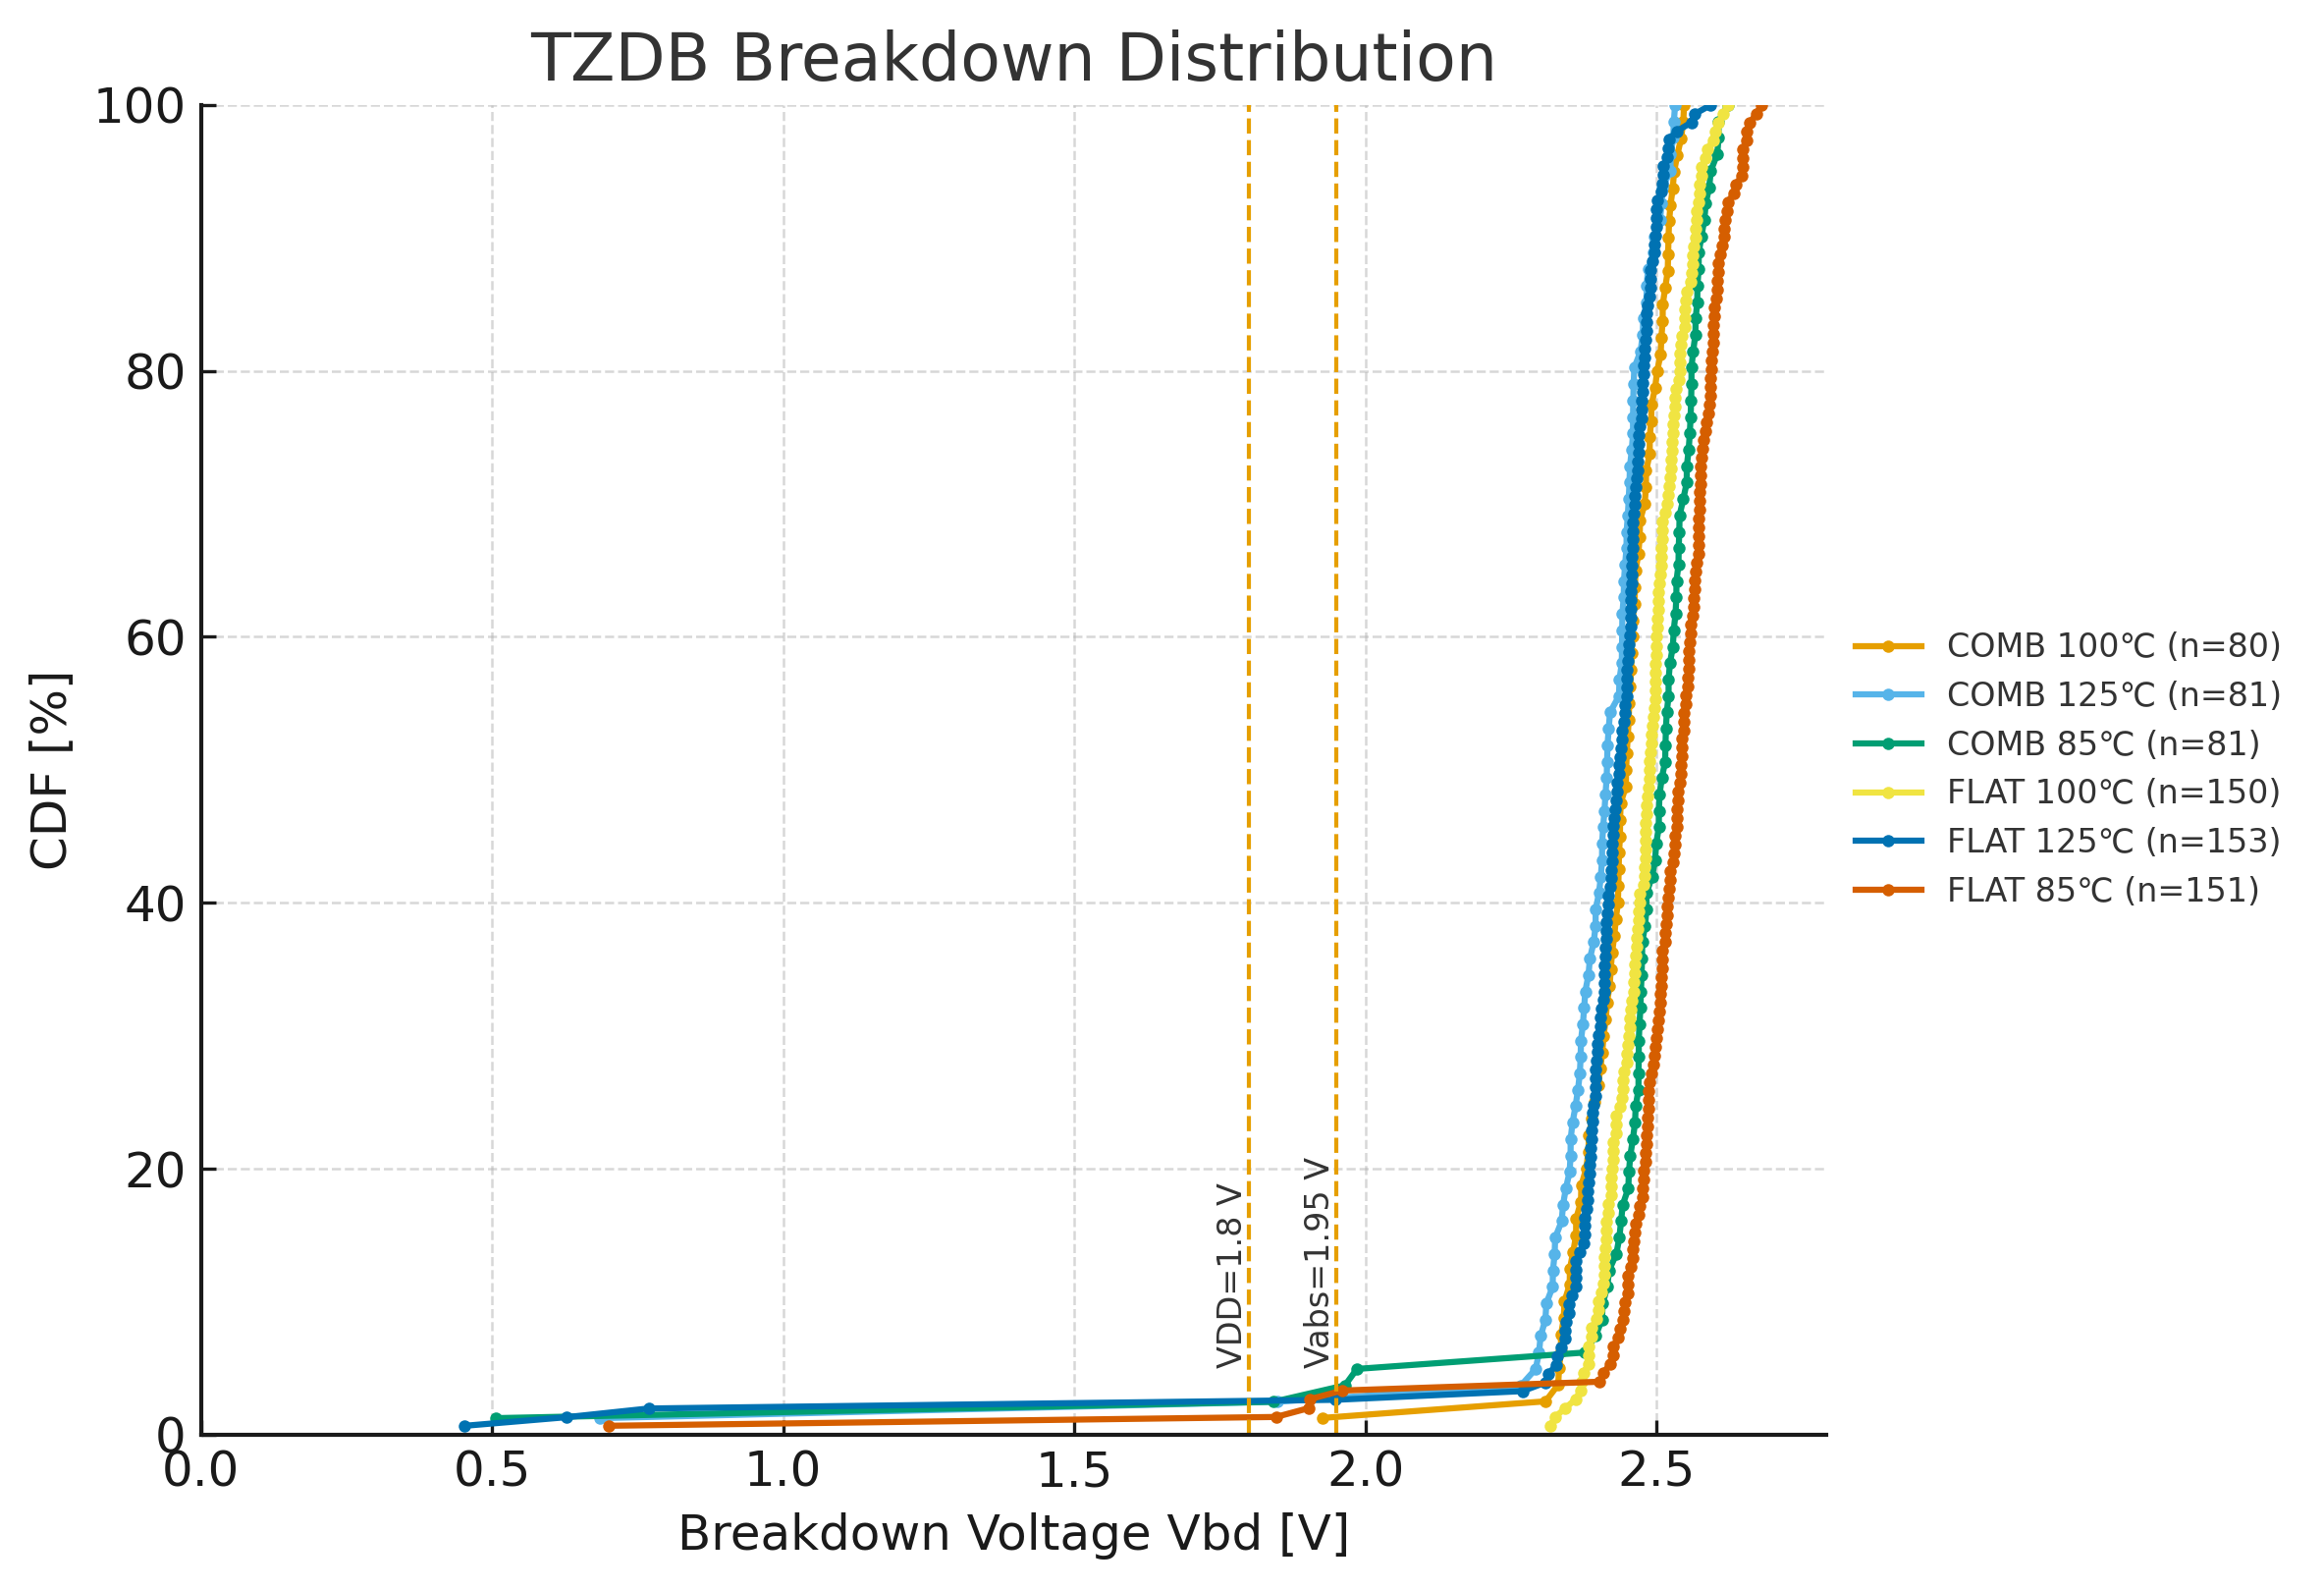
\includegraphics[width=\linewidth]{figures/fig3_tzdb.png}
\caption{TZDB distributions of FeCAPs.}\label{fig:tzdb}
\end{figure}
}{}

\subsection{TDDB (Weibull/Arrhenius)}
Weibull analysis yields \(\beta \approx 1.3\) across stress conditions.
\IfFileExists{figures/fig4_tddb_cdf.png}{%
\begin{figure}[t]\centering
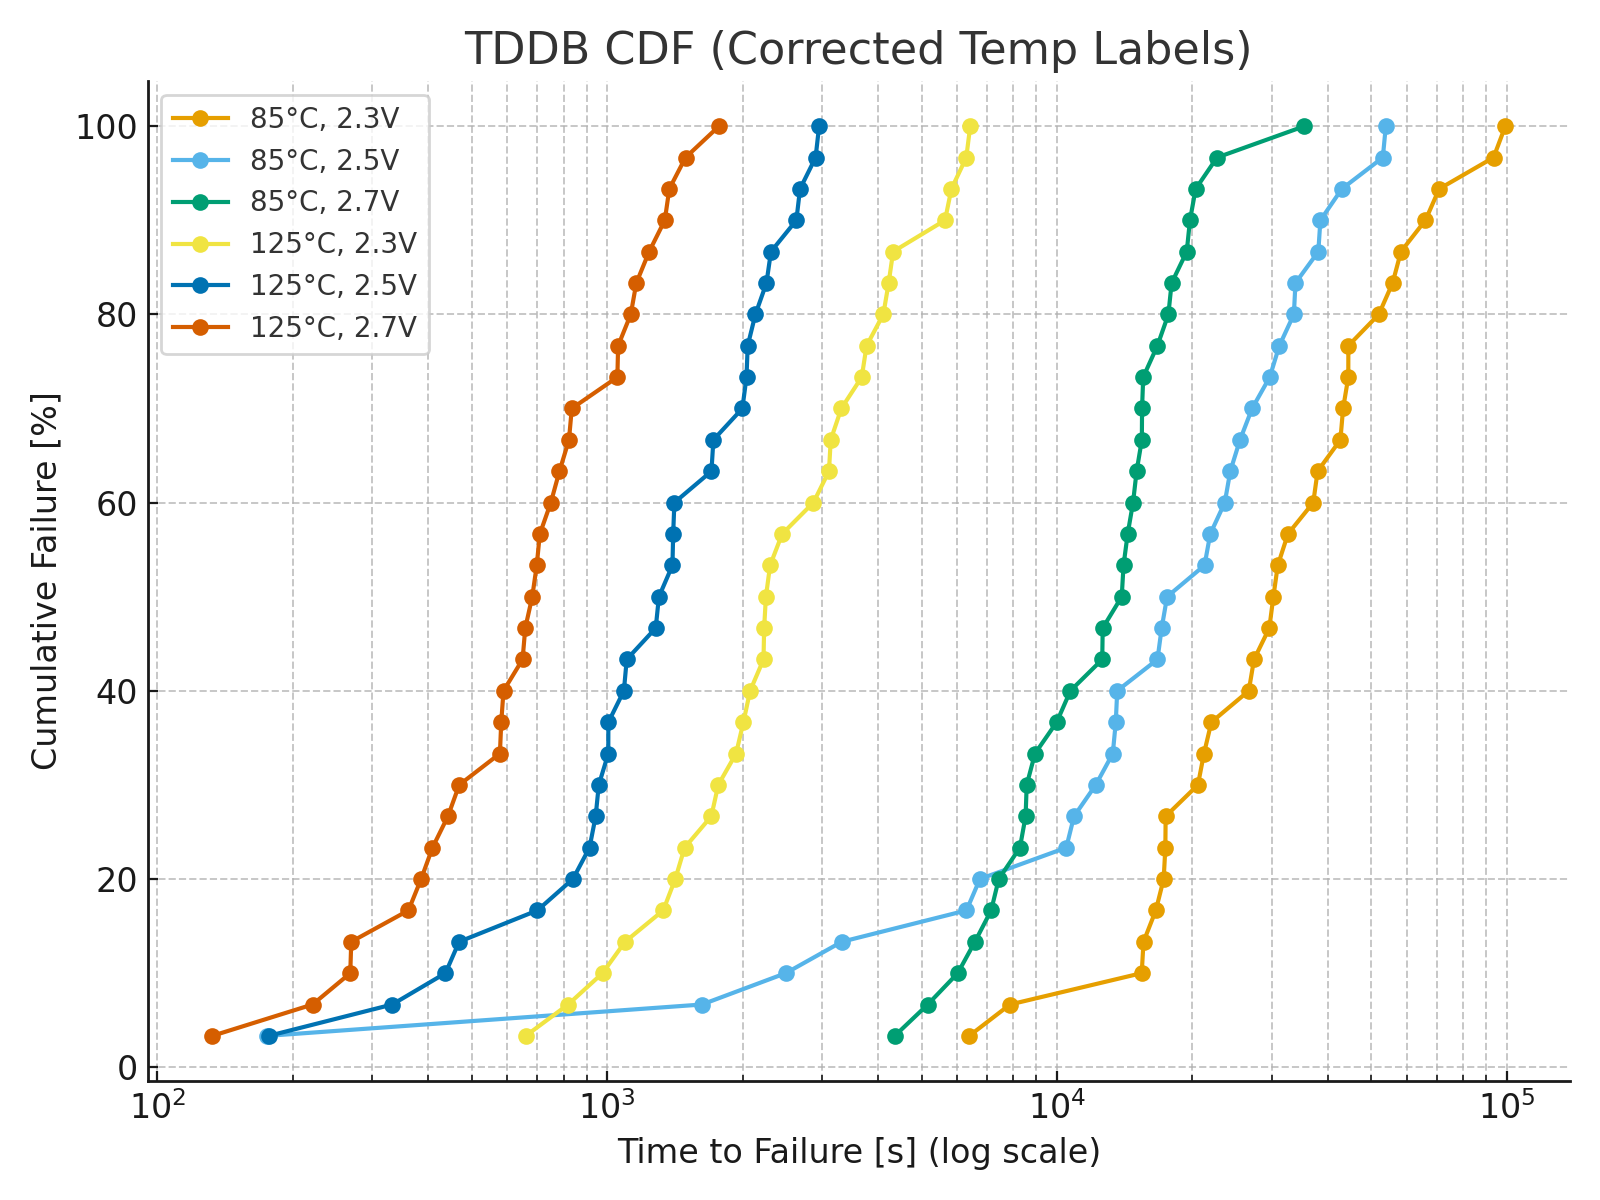
\includegraphics[width=\linewidth]{figures/fig4_tddb_cdf.png}
\caption{TDDB CDF for all stress conditions.}\label{fig:tddb_cdf}
\end{figure}
}{}
\IfFileExists{figures/fig4_tddb_weibull.png}{%
\begin{figure}[t]\centering
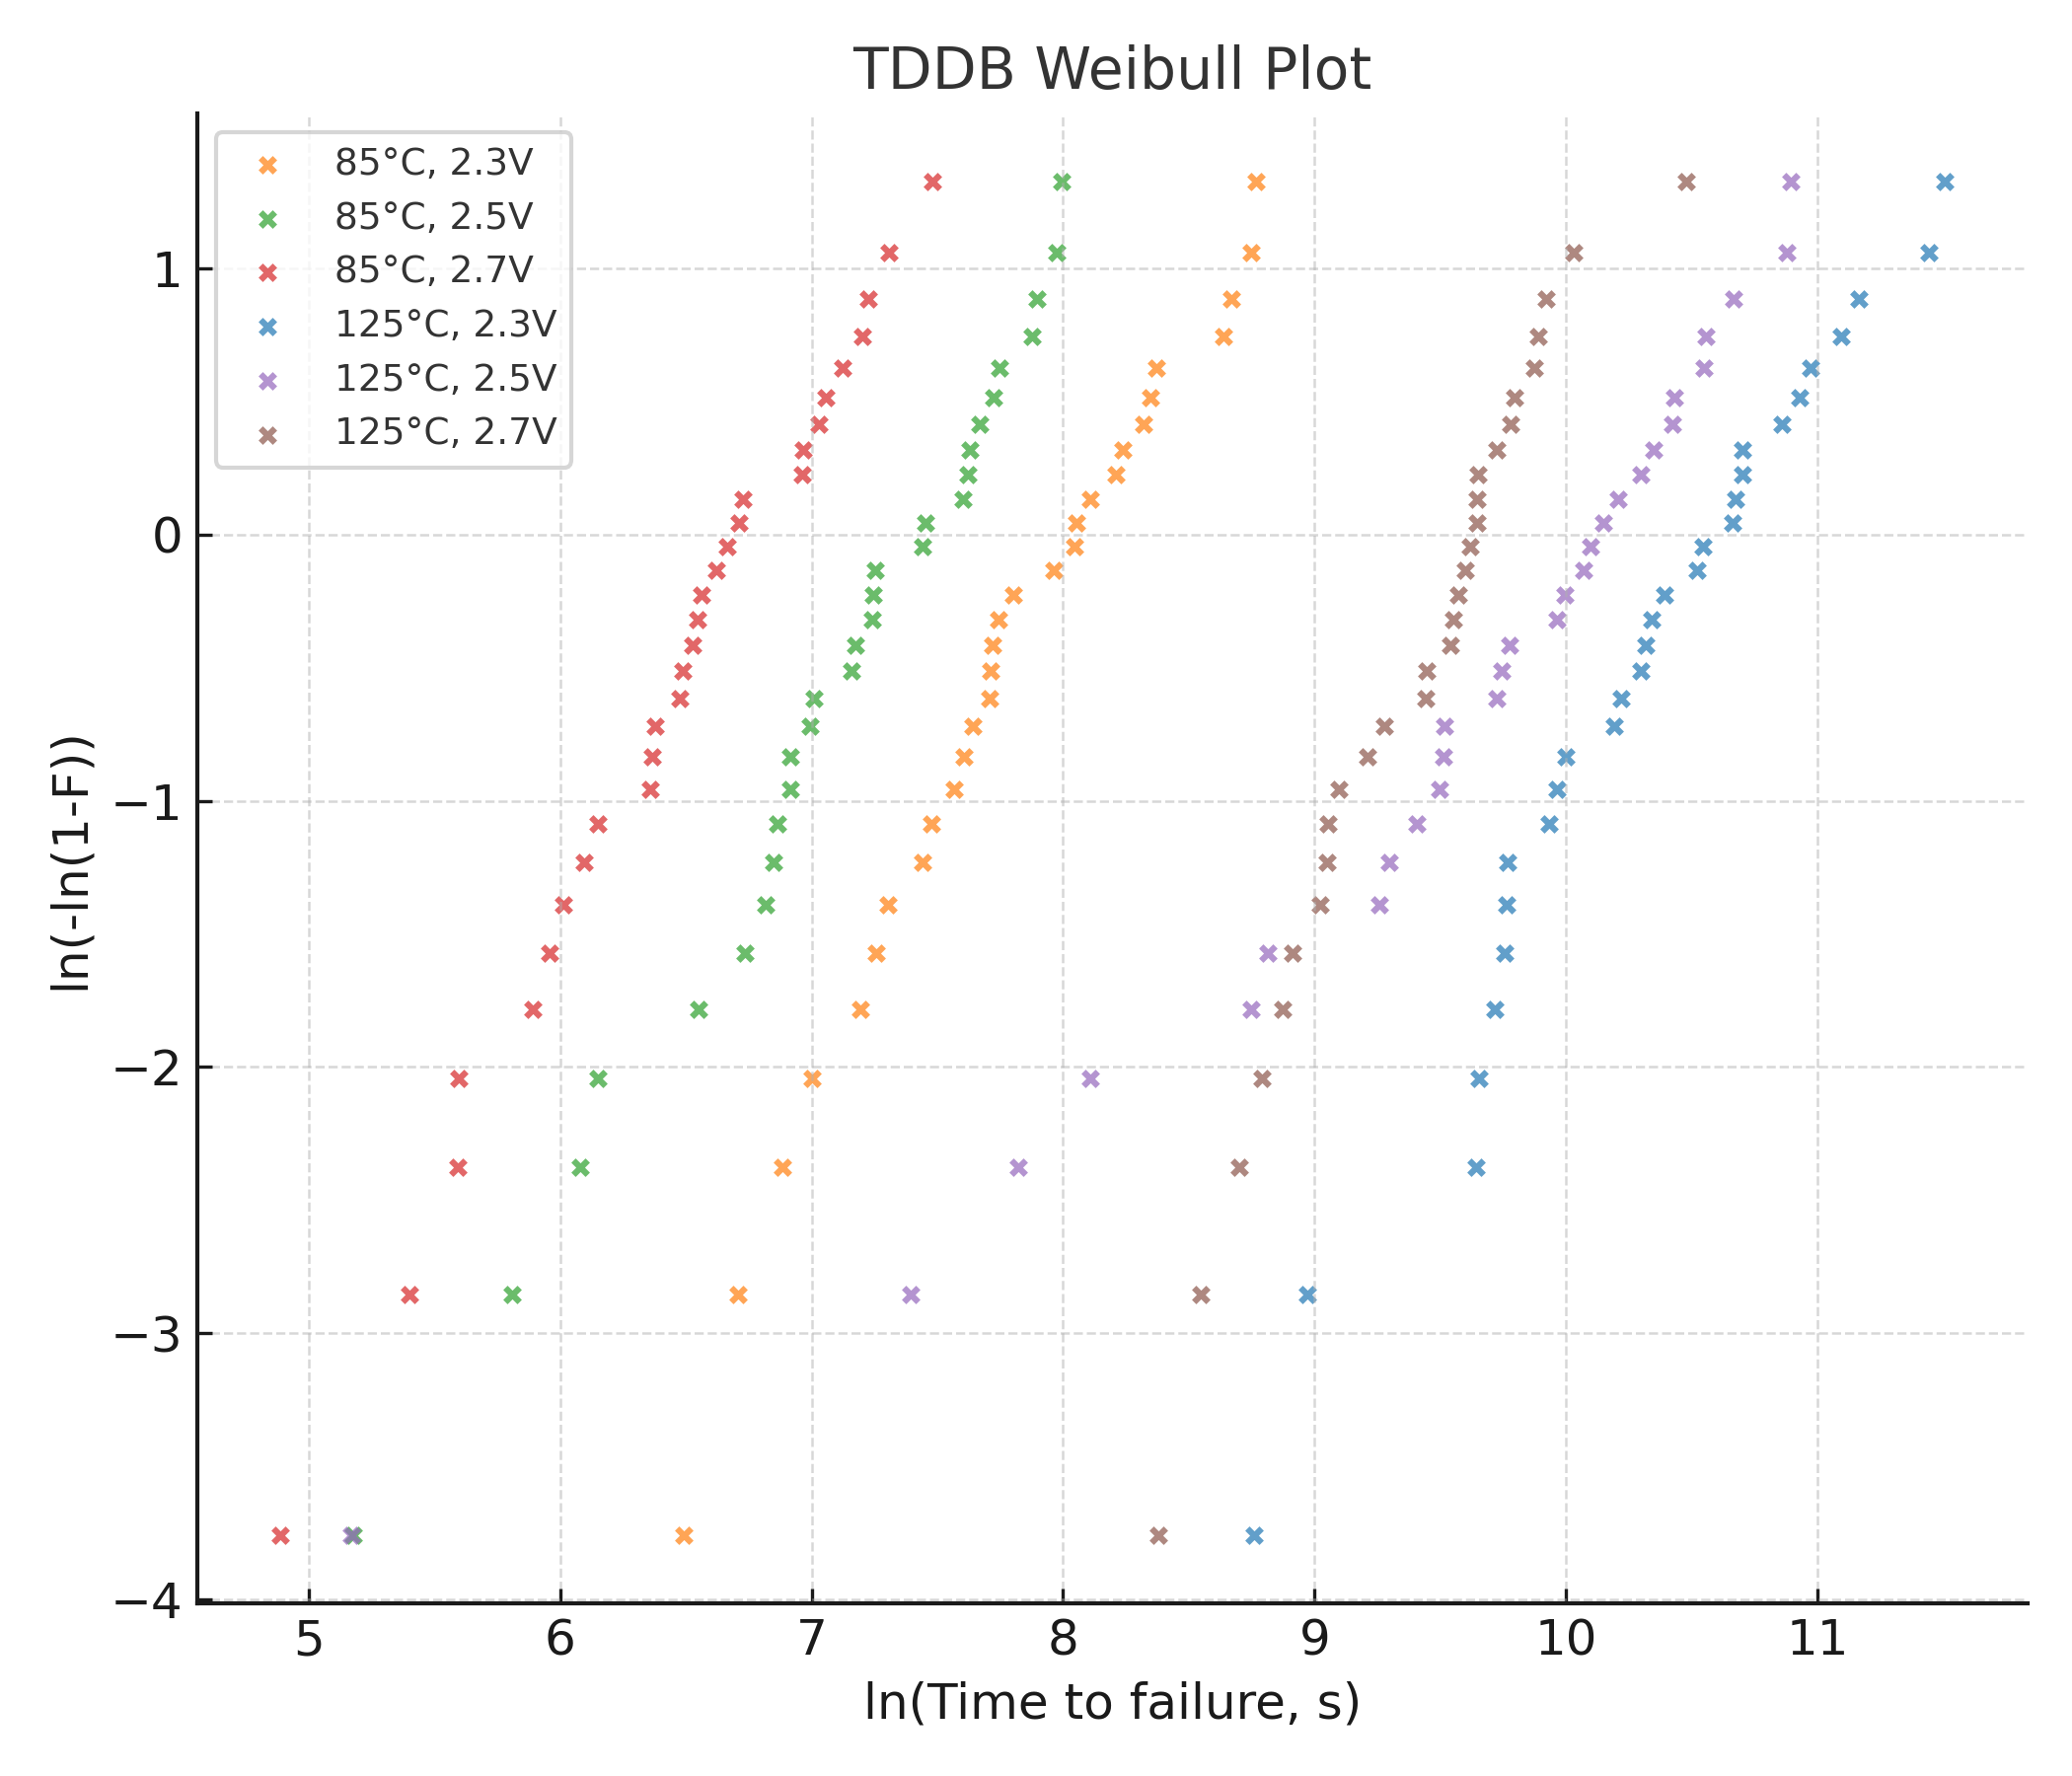
\includegraphics[width=\linewidth]{figures/fig4_tddb_weibull.png}
\caption{TDDB Weibull plots with fitted lines (\(\beta,\eta\)).}\label{fig:tddb_weibull}
\end{figure}
}{}

From the fitted scales \(\eta\), Arrhenius fitting gives activation energies consistent with oxygen-vacancy diffusion:
\(E_a \approx 0.78\)~eV (@2.3~V), \(0.84\)~eV (@2.5~V), \(0.88\)~eV (@2.7~V).
A compact summary is listed in Table~\ref{tab:tddb_eta}.

\begin{table}[t]
\centering
\caption{Extracted TDDB scales \(\eta\) (representative) and conditions.}
\label{tab:tddb_eta}
\begin{tabular}{@{}lcc@{}}
\toprule
Condition & Temp & \(\eta\) [s]\\
\midrule
2.3 V & \SI{85}{\celsius} & \(2.7\times10^{3}\) \\
2.3 V & \SI{125}{\celsius} & \(5.1\times10^{4}\) \\
2.5 V & \SI{85}{\celsius} & \(1.5\times10^{3}\) \\
2.5 V & \SI{125}{\celsius} & \(2.8\times10^{4}\) \\
2.7 V & \SI{85}{\celsius} & \(8.2\times10^{2}\) \\
2.7 V & \SI{125}{\celsius} & \(1.5\times10^{4}\) \\
\bottomrule
\end{tabular}
\end{table}

\subsection{Endurance}
Up to \(10^{5}\) cycles were verified; the threshold window \(\Delta V_{\mathrm{th}}\) shrinks by roughly 20–30\%.
A simple fit \(\Delta V_{\mathrm{th}}(N)=1.12-0.05\log_{10}N\) matches the trend.
\IfFileExists{figures/fig5_endurance.png}{%
\begin{figure}[t]\centering
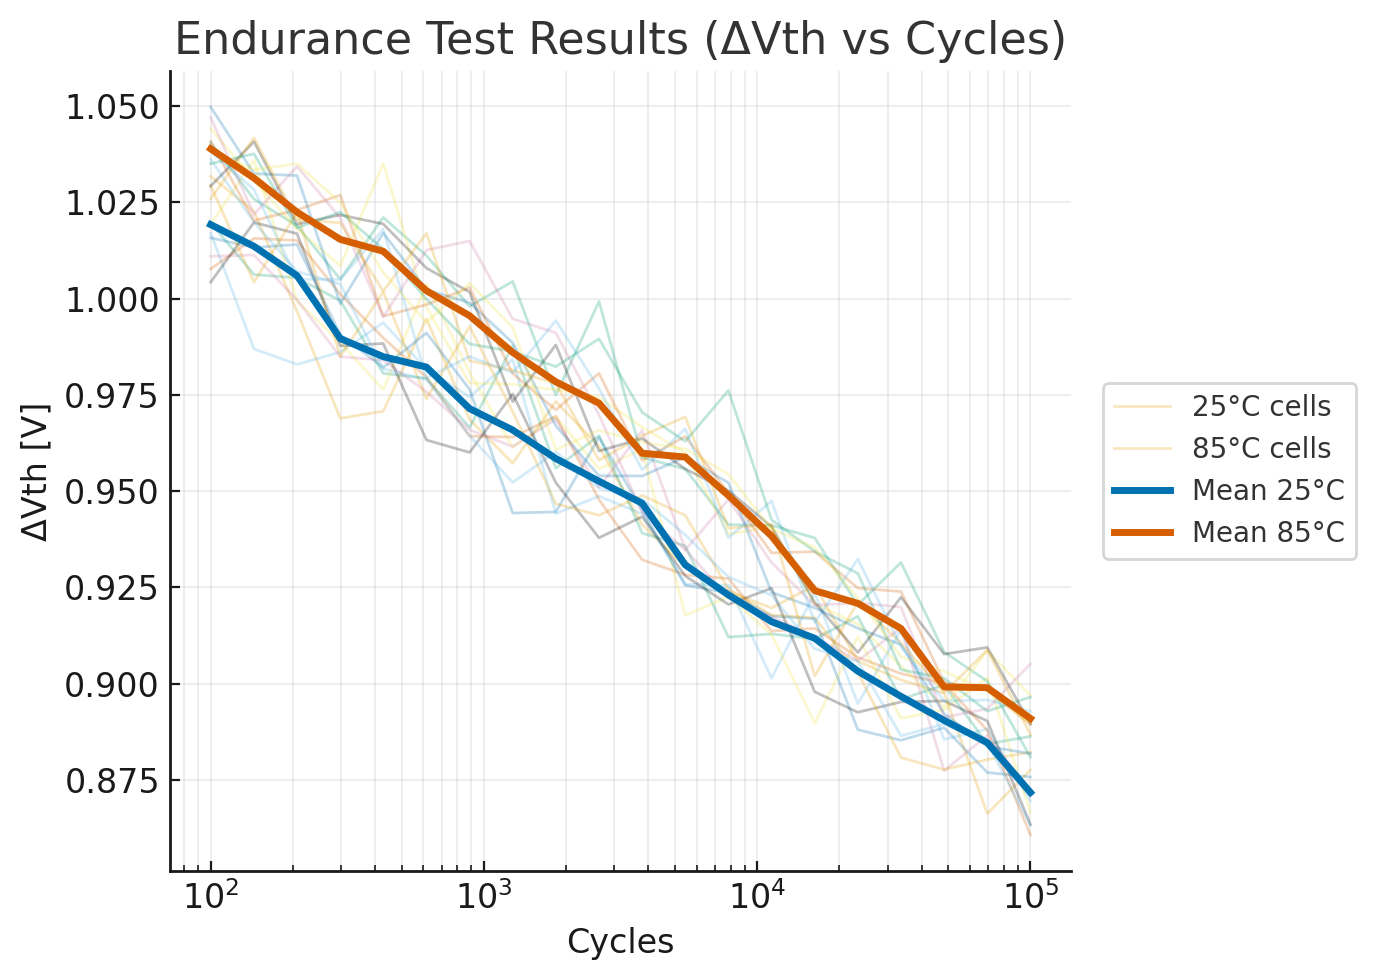
\includegraphics[width=\linewidth]{figures/fig5_endurance.png}
\caption{Endurance characteristics (\(\Delta V_{\mathrm{th}}\) vs. cycles).}
\label{fig:endurance}
\end{figure}
}{}

\subsection{Retention (Automotive View)}
Arrhenius extrapolation with \(E_a\approx 1.1\)~eV predicts:
\(>\!10^{2}\)~years at \SI{25}{\celsius}, \(>\!10\)~years at \SI{85}{\celsius} (Grade-2), but only months at \SI{150}{\celsius}.
\IfFileExists{figures/fig6_retention.png}{%
\begin{figure}[t]\centering
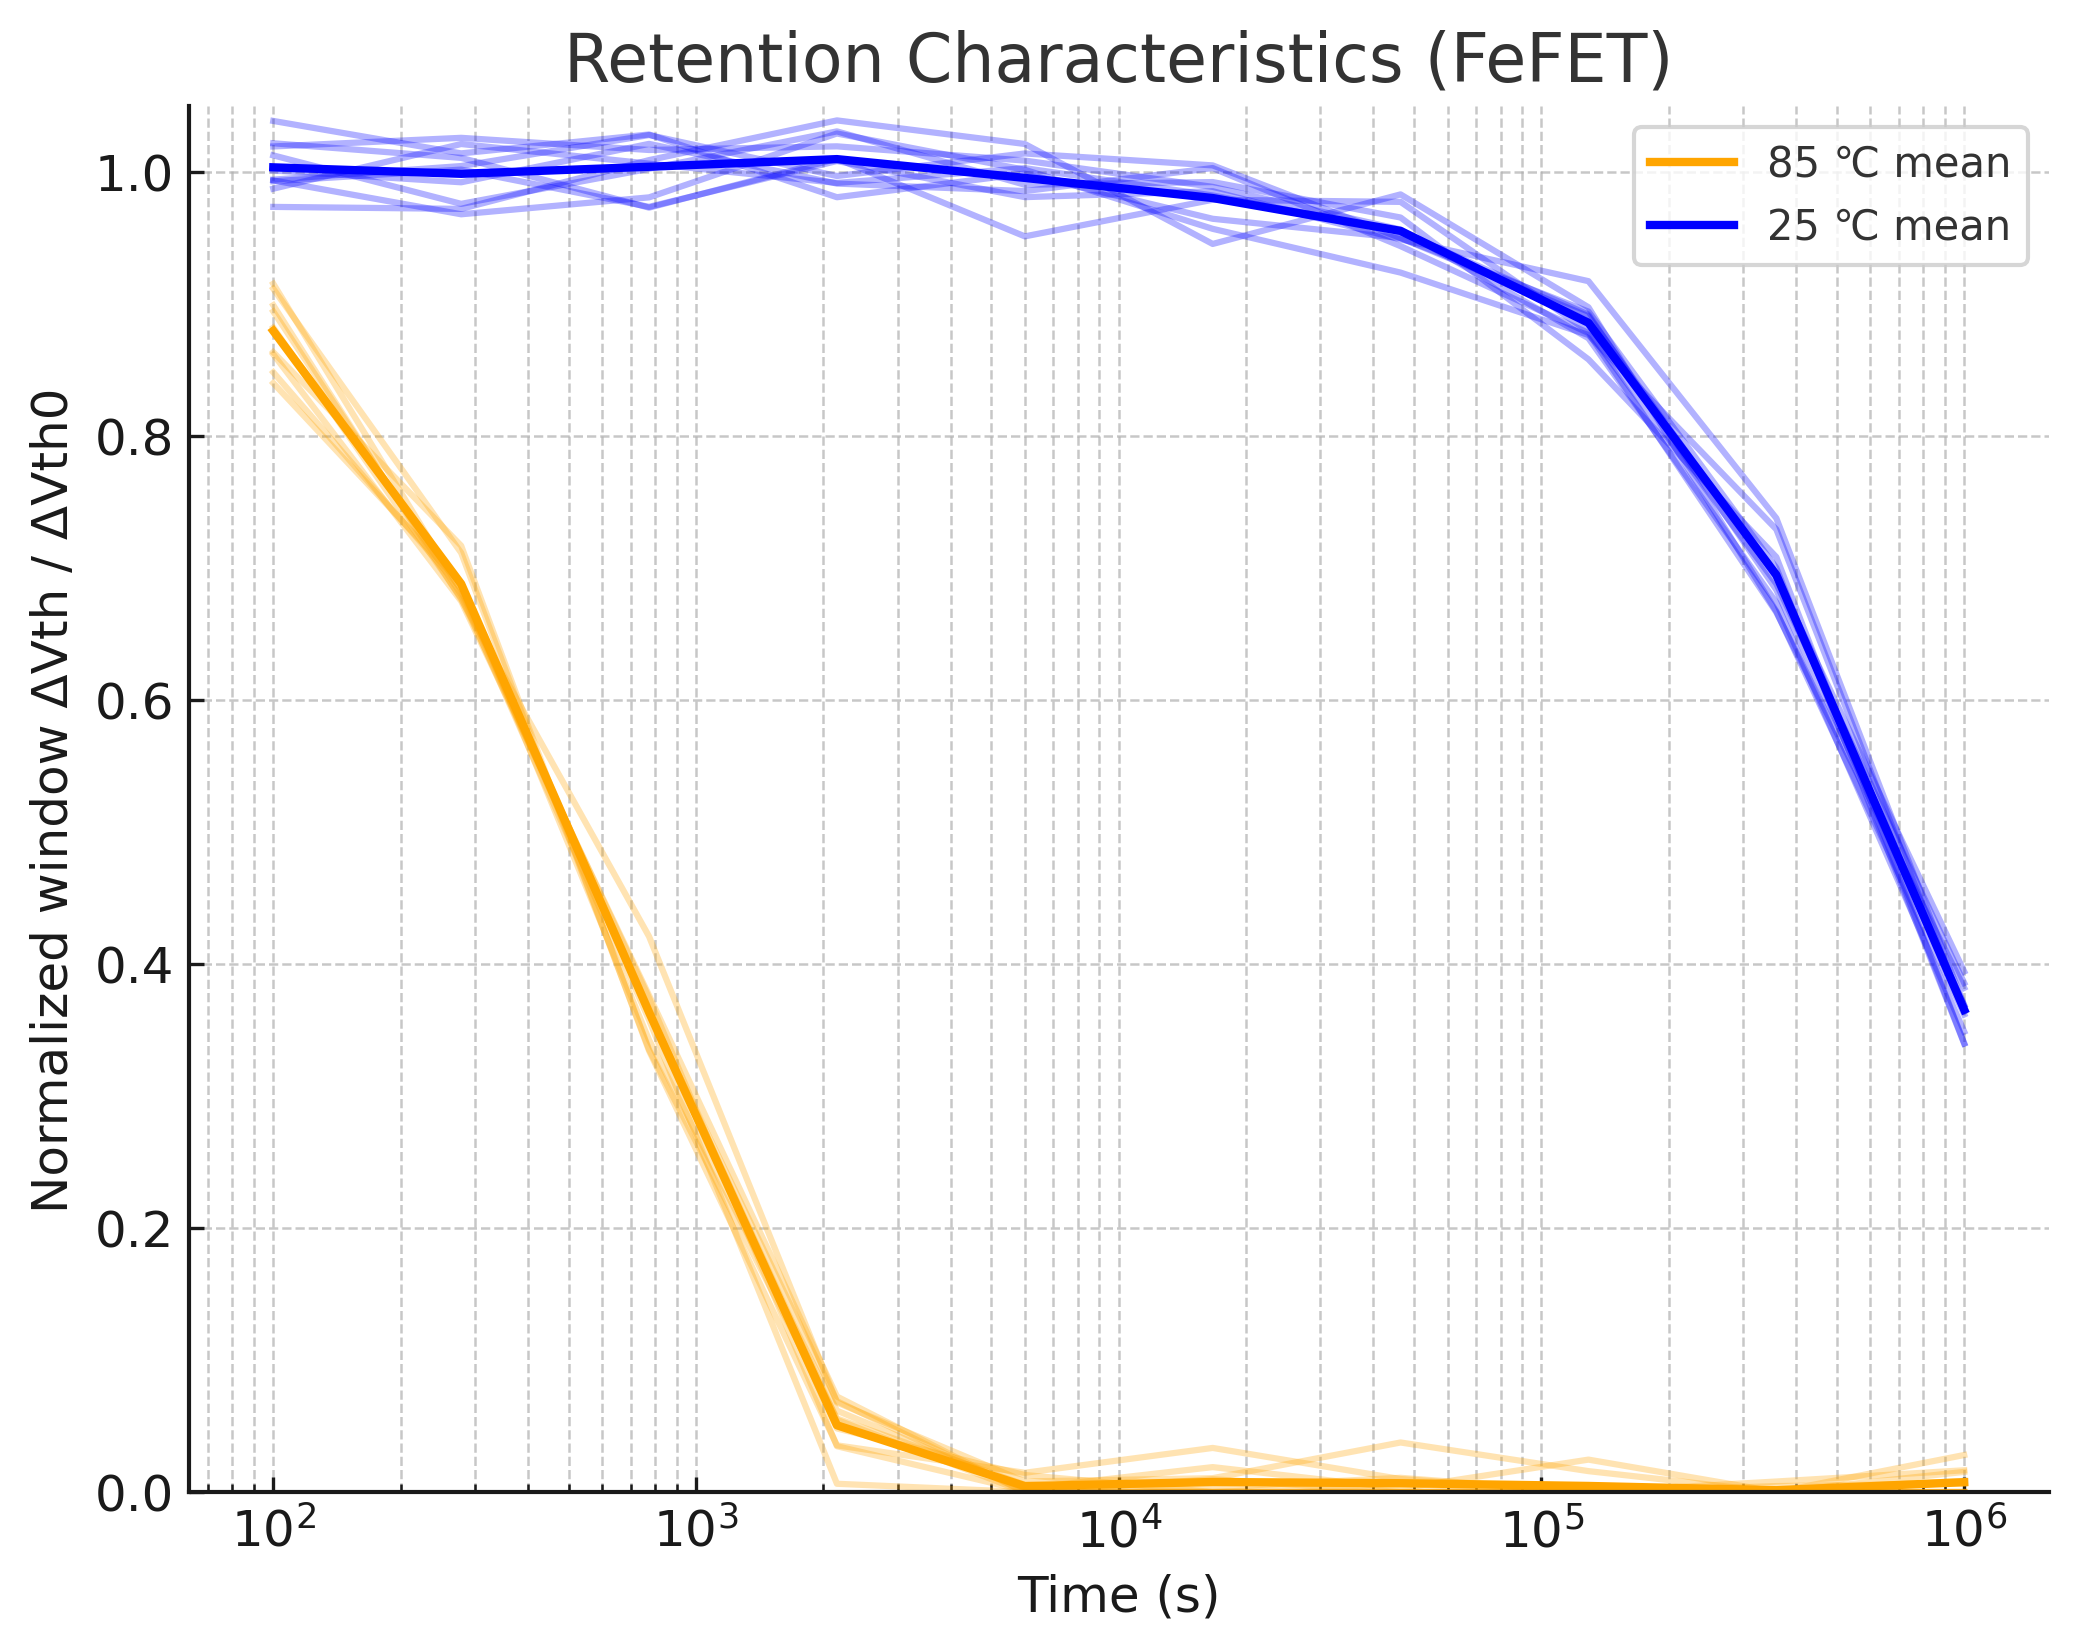
\includegraphics[width=\linewidth]{figures/fig6_retention.png}
\caption{Retention characteristics and Arrhenius extrapolation.}
\label{fig:retention}
\end{figure}
}{}

\section{System Architecture (SRAM + FeFET)}
The core domain operates at \SI{1.8}{V} (logic, SRAM, and FeFET). FeFET write pulses (\(\pm 2.5\)~V, \SI{1}{--}\SI{50}{\micro s}) are generated by an on-chip charge pump. A controller transfers SRAM contents to FeFET upon power-fail detection and restores them on power-up. An optional \SI{3.3}{V} peripheral domain serves I/O and AMS blocks.

\IfFileExists{figures/system_arch_block.png}{%
\begin{figure}[t]\centering
\includegraphics[width=\linewidth]{figures/system_arch_block.png}
\caption{Block-level system architecture: 1.8-V core with SRAM+FeFET and charge pump; optional 3.3-V periphery.}
\label{fig:sys}
\end{figure}
}{}

\IfFileExists{figures/backup_restore_flow.png}{%
\begin{figure}[t]\centering
\includegraphics[width=\linewidth]{figures/backup_restore_flow.png}
\caption{Backup/restore path between SRAM and FeFET with power-fail detection.}
\label{fig:backup}
\end{figure}
}{}

\section{Discussion}
The HZO/Al\(_2\)O\(_3\)/TiN stack provides sufficient reliability for industrial/consumer embedded NVM. For high-temperature automotive, improvements are required: (i) IL thickness optimization and HZO crystallinity control, (ii) refresh/rewrite operation, and (iii) ECC and redundancy.

\section{Conclusion}
We realized an FeFET module on \SI{0.18}{\micro m} CMOS with only \textbf{one extra mask} and \textbf{one ALD tool}. Devices exhibit \(>10^{5}\) cycles and \(>\!10\)~years retention at \SI{85}{\celsius}. The method extends mature-node lifetime and enables cost-effective embedded NVM for automotive/industrial/IoT, while high-temperature retention remains the key item for Grade-1/0.

\section*{Acknowledgment}
The author thanks collaborators for helpful discussions.

\bibliographystyle{IEEEtran}
\begin{thebibliography}{99}
\bibitem{Boscke2011} T.~Böscke \emph{et al.}, \emph{Appl. Phys. Lett.}, vol.~99, p.~102903, 2011.
\bibitem{Mueller2012} J.~Müller \emph{et al.}, \emph{Appl. Phys. Lett.}, vol.~99, p.~112901, 2012.
\bibitem{Mikolajick2019} T.~Mikolajick \emph{et al.}, \emph{J. Appl. Phys.}, vol.~125, p.~204103, 2019.
\bibitem{Mueller2015} J.~Müller \emph{et al.}, \emph{IEEE Trans. Electron Devices}, vol.~62, no.~12, pp.~4158--4166, 2015.
\bibitem{Park2020} J.~Park \emph{et al.}, \emph{IEEE Electron Device Lett.}, vol.~41, no.~5, pp.~711--714, 2020.
\bibitem{Nakamura2003} H.~Nakamura \emph{et al.}, \emph{IEEE Trans. Device Mater. Rel.}, vol.~3, no.~4, pp.~132--136, 2003.
\bibitem{Yamazaki2018} K.~Yamazaki \emph{et al.}, \emph{Jpn. J. Appl. Phys.}, vol.~57, 04FB07, 2018.
\end{thebibliography}

% --- Optional biography section (IEEEtran conferences often omit biographies)
\section*{Biography}
\textbf{Shinichi Samizo} has over 25 years of experience in semiconductor process integration and actuator development. After studying control theory and EM modeling in academia, he joined Seiko Epson in 1997 and worked on 0.35--0.18~\(\mu\)m logic/memory/HV CMOS integration, including DRAM process ramp, HV-to-logic integration, and LCD driver products. Later he contributed to PZT actuator development and the PrecisionCore inkjet head. He is currently an independent researcher focusing on semiconductor process integration and actuator/system education via the “Project Design Hub”.
\end{document}
